\chapter{Introduction de l'équipe}

Notre équipe est composée de 8 personnes:

\paragraph{Joey Brynckman} (Serveur marchand, application Android \& bases du National Bank Server)

Je me suis occupé principalement de la partie marchande de notre application. J'ai donc créé le serveur
permettant de contenir les données relatives aux comptes et aux produits à vendre. Pour ce faire, je me
suis donc occupé de la création de la base de données, de l'accès à ses données grâce à un ORM, de l'API
et de la sécurisation de ses endpoints.

Comme le National Bank Server fonctionne sur un principe similaire au serveur marchand, je me suis
donc également occupé de ces aspects de ce serveur. Bien sûr, pour le NBS, il y a beaucoup plus à faire
que ça, notamment l'accès aux bases noSQL et la génération de données, mais c'est Thibault qui s'est
occupé de ces parties-là. Je n'ai fait que la base de ce serveur.

Enfin, je me suis également occupé de l'application Android. Ses pages, leur fonctionnement, ainsi que
les accès à l'API du serveur que j'ai créé. Seule la page de paiement n'a pas été faite par moi, comme il
s'agit d'une page web, d'un portail de paiement créé par Lionel.

Mon choix de faire ces parties vient du fait que j'avais moi-même commencé un projet personnel qui
fonctionnait de manière similaire à notre application Android et notre serveur marchand. J'avais donc
certaines bases et connaissances que j'ai pu utiliser à bon escient.

\paragraph{Andrea Dal Molin} (Responsable Java Card \& beID)

L'intégration de l'authentification via carte d'identité électronique et la gestion des cartes de fidélité ont été mes principales tâches au sein du groupe. Les raisons de ce choix se justifient par la possession personnelle du matériel utile au développement de ces parties, notamment pour ce qui concerne la lecture de carte d'identité électronique. 

De plus, je portais personnellement un intérêt particulier quant à l'intégration de ces deux technologies différentes avec une architecture complète comme celle du Projet Intégré. Comme il sera décrit dans la partie concernant mes sujets, le développement des parties s'est révélé stimulant. 

\paragraph{Thibault Havet}
\paragraph{Flo Raeymaeckers} (DevOps \& Responsable Équipe)

Je me suis occupée de l'infrastructure logicielle du déploiement de la solution. Plus précisément, j'ai mis en place un cluster de serveurs afin que l'ensemble des services que l'on voulait déployer sur le serveur puisse profiter d'un load balancing et d'une virtualisation par container afin d'avoir une scalabilité horizontale des services en fonction de la demande.

De plus, j'ai géré l'équipe. J'ai travaillé sur la mise en commun des ressources (réunions, outils de suivi de projet...), de ce rapport, et enfin de la présentation que vous allez pouvoir assister. Je vais passer en revue dans ce document les différentes difficultés par lesquelles je suis passée et les éventuelles solutions que j'ai apporté.

\paragraph{Arnaud Rase} (Responsable réseau \& aide en DevOps)

Pour ma part, j'ai été mit en charge de l'implémentation de la partie sur le réseau privé de la
banque Picsou. J'ai également aidé Florent à lier celle-ci aux différents serveurs hébergés sur
l'ESXi. L'infrastructure aura 2 grandes parties, la partie routage et switching, nous pourront
notamment retrouver du load balancing, de la traduction d'adresses IP publiques en adresses
IP privée et une disponibilité presque ininterrompue

\paragraph{William Tea}
\paragraph{Lionel Thys}
\paragraph{Alexandre Villance} (Responsable NoSQL)

J'ai pris en charge la mise en place des bases de données dans le projet. Mon attention s'est
principalement portée sur la partie NO-SQL, et nous avons choisi d'utiliser MongoDB en le combinant
avec Docker. J'ai configuré plusieurs replica sets et mis en place le sharding. J'ai également collaboré
avec les personnes chargées de stocker les données dans la base de données, en assurant une bonne
communication pour assurer leur bon fonctionnement

\chapter{Étude et mise en théorie de l'infrastructure}

Dans ce chapitre, nous allons passer en revue l'étude que nous avons effectué sur l'énoncé du projet transmit pas nos professeurs. Le projet part d'un énoncé basé sur une version "simplifiée" de 3D secure, ou du moins plus ou moins cousine: nous avons un marchand qui souhaite pouvoir proposer à ses clients la vente de ses services/bien en ligne. Afin que le consommateur puisse payer, le marchand a besoin d'une plateforme de paiement en ligne. Notre rôle est d'implémenter cette plateforme de payement au niveau de la banque du consommateur, qui va alors se synchroniser avec la banque du marchand pour valider la transaction.

\section{Schéma de l'infrastructure}

\begin{figure}[H]
    \centering
    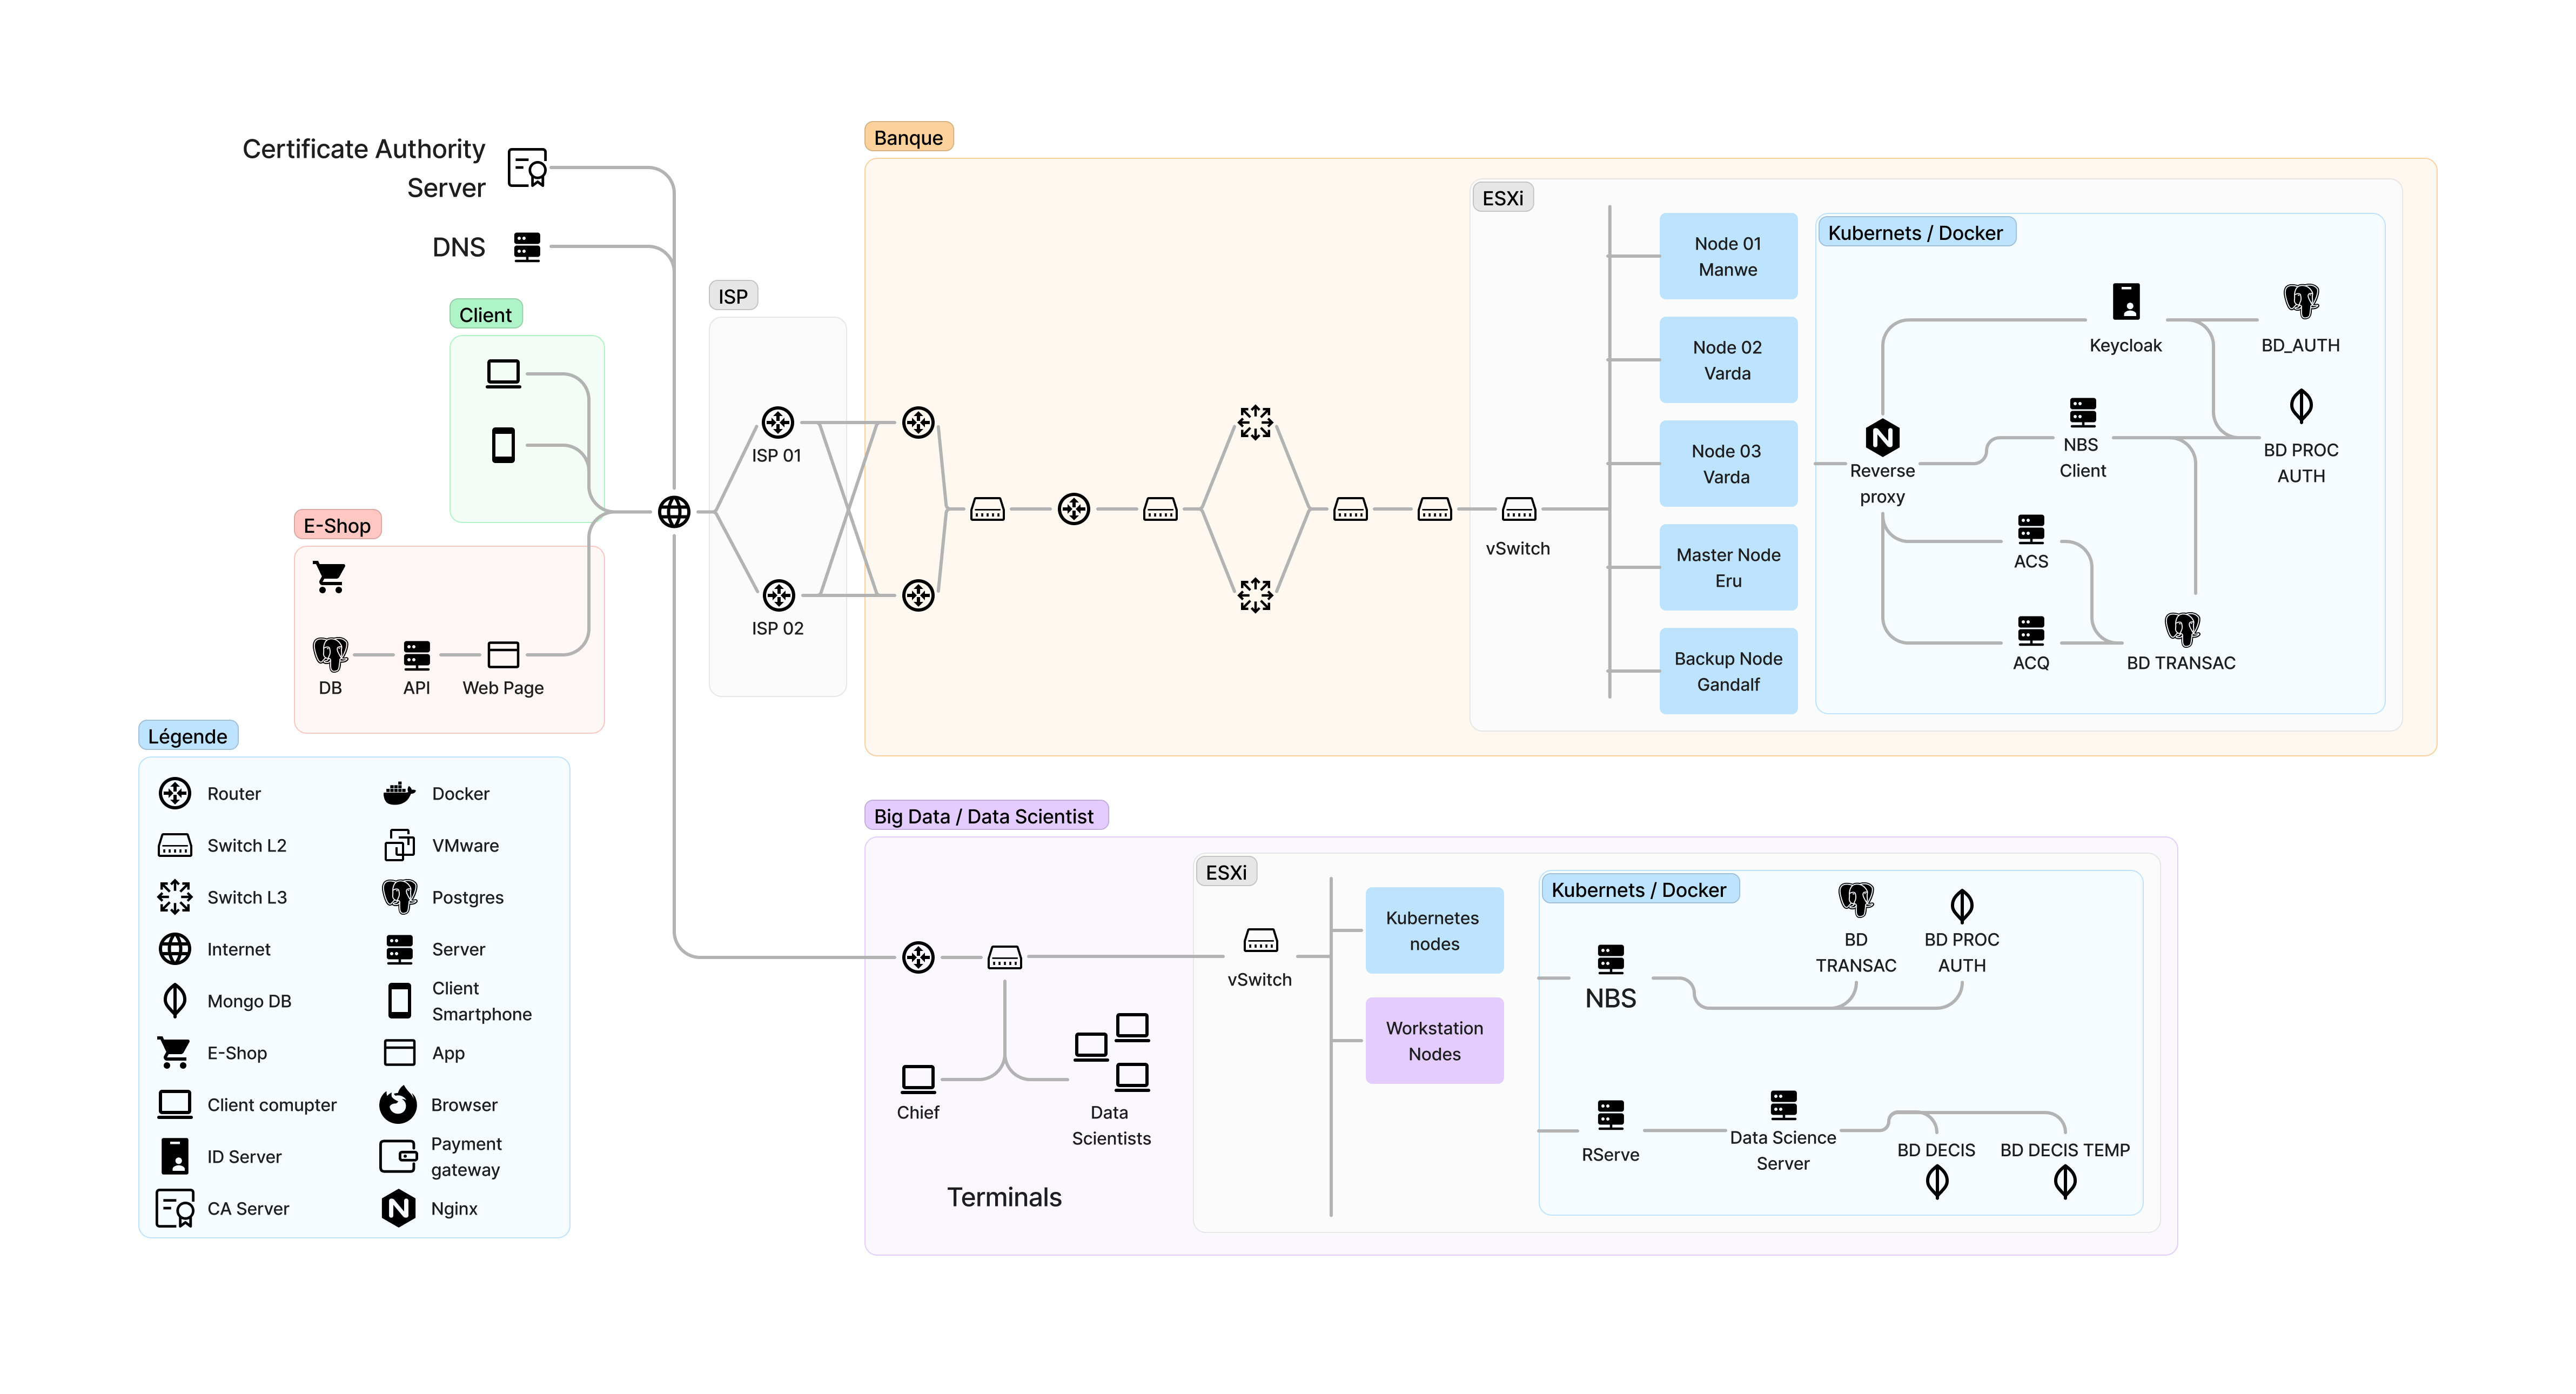
\includegraphics[width=\textwidth]{./img/Schéma Projet Intégré.png}
    \caption{Schéma global du projet intégré}
    \label{fig:infrastructure}
\end{figure}